
\chapter{Validation}
\section{Validation Strategy}
Model validation could be considered an important step towards creating a robust and useful simulation tool, though there is little dedicated literature referring to the process of successfully validating wave solving acoustic simulation software. A greater volume of literature is availalbe for the validation of Ray based methods such as~\cite{Ahnert2005,Tsingos2002}, and the validation of a hybrid scheme by Murphy \textit{et al} is available ~\cite{Southern2013}. Studies such as Hill~\cite{Hill2012}. This section will review an attempt to validate the FDTD and PSTD tools described above, with a small 3D domain.\\

\subsection{The Domain}
The domain used for validation in this study was a fully bounded room with the following properties:\\

\begin{itemize}
\item Length $L_x = 5m$
\item Width $L_x = 4m$
\item Height $L_z = 3m$
\item Volume = $ v = 60m^3$
\item Surface Area $S_{area} = 94m^2$
\item Uniform Absorption Coefficient $\alpha = 0.45 $
\item Schroeder Frequency  $f_{schroeder} = 107Hz $,
\item The Reflection Order $N_{reflections} = 30.7$
\item Mean Free Path Between Reflections $MFP = 2.55m$
\item Eyring Reverberation Time $RT_{60} = 0.1719s $
\end{itemize}

The axial, tangential and oblique modes below the Schroeder frequency are calculated as:\\


The stimulus position in each domain was $1.0m$ in each direction from the bottom left corner, and the receiver position was the exact middle of the domain. The stimulus source type was a soft source, as described in the time domain numerical methods section above. The source content was a log chirp that was generated using the Matlab DSP Systems Toolbox, with a start frequency of 100Hz and a stop frequency of half the maximum target frequency (or a quarter of Nyquist), that was normalised to $100dBSPL$ and has a sweep time of $0.4s$. Before normalisation, a Hann window was applied to the signal to minimize the discontinuity of introducing the source. The maximum frequency of interest in this validation was $5kHz$, giving a $0.333e^{-5}$ step time for the FDTD simulation, and a $0.1e^{-4}$ step time for the PSTD simulation. A plot of the source signal amplitude with respect to time is given below:\\

\subsection{Post Processing}
The aim of the validation will be to show that there is minimal error in the normalised power spectral density between source and receiver location. This will show that waves are travelling from source to receiver with minimal error i.e. without aliasing or unexpected loss in the frequency range of interest. Some modal influence is expected, as is DC offset. To reduce the effect of the dc term, a DC blocking filter will be used when post processing the source and receiver recorded signals.

\section{Results}
Below is a plot of the spectral power of the source signal, the FDTD receiver position and the PSTD receiver position for the simulation described above. The receiver signals are normalised the maximum of the source position amplitude, as described in~\cite{Murphy2014}.\\ 


\begin{figure}[H]
\centering
  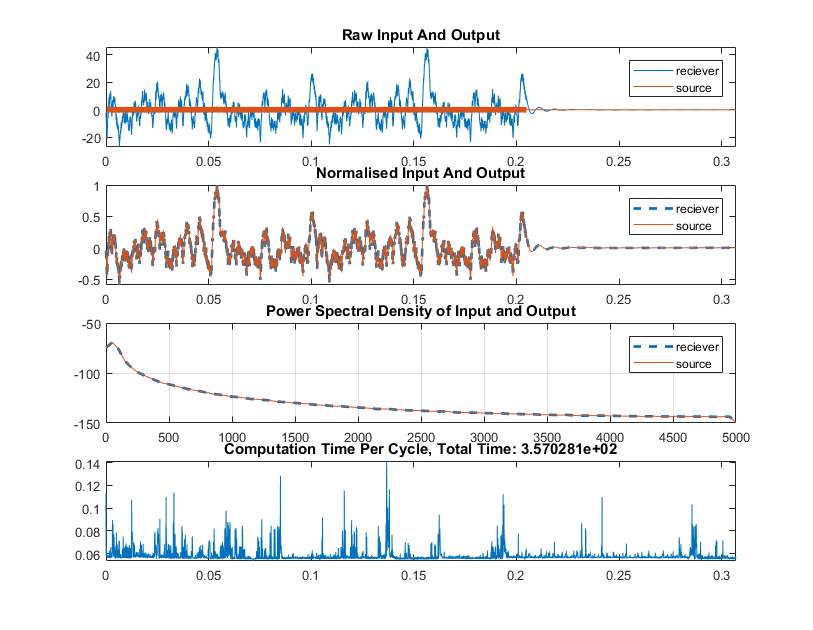
\includegraphics[width=\textwidth]{./graphics/PSTDvalidation10k.png}
  \caption{Validation data of PSTD simulation}
\end{figure}

It can be seen that both simulations exhibit similar inclusion of the frequency domain properties of the stimulus. Both simulations include the dip from Dc to 55Hz, and both exhibit the slope from 2400Hz that is caused by the window function. However, the PSTD results include a considerable spectral tilt, which may be partially caused by the implementation of a soft source as opposed to a transparent source.\\


\section{Validating The SFDTD Method}
As noted previously, the SFDTD method was implemented only to 2D and thus cannot be validated against he performance of the 3D FDTD and PSTD methods as above. Below is a comparative plot of the SFDTD receiver signal and the source signal. The threshold for windowing of the SFDTD algorithm was set to 30dB.\\

As can be seen in the plot above, though the frequency content of the received signal is similar to the source, there is a continually increasing noise level that may be caused by the discontinuity of the fluctuating mask. Due to this noise level it is not appropriate to successfully validate this simulation method, as so the inclusion of this method in the next section is purely to explore the potential of the method.\\ 